\chapter{Motiva\c tie}\footnote{Proiectul s-a derulat \^ in cadrul \c si cu sprijinul Laboratorului de \textbf{CE}rcetare \^ in domeniul \textbf{R}ealit\u a\c tii \textbf{V}irtuale \c si \textbf{A}ugmentate (CERVA). Pentru detalii vizita\c ti: http://www.univ-ovidius.ro/cerva.}

\section{Sec\c tiune}
\subsection{subsec\c tiune}

Text demonstrativ pentru diacritice:

\^ i \^ I \^ a \^ A \c s \c S \c t \c T \u a \u A 

Demo figura \ref{fig:demo1} \c si o citare din fi\c sierul refs.bib \cite{albeanu05}.

\begin{figure}[htbp]
	\centering
		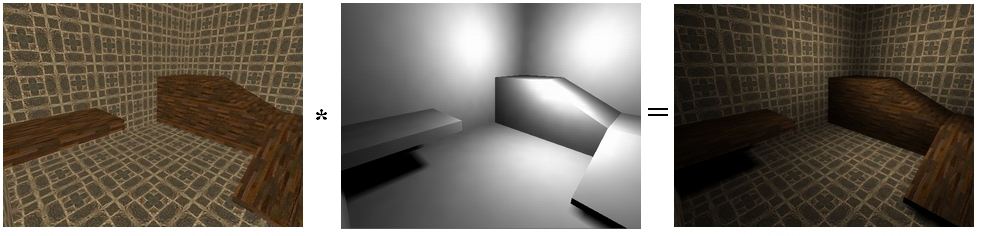
\includegraphics[scale=0.40]{all.jpg}
	\caption{Explica\c tie figur\u a.}

\label{fig:demo1}
\end{figure}

\begin{figure}[htbp]
	\centering
		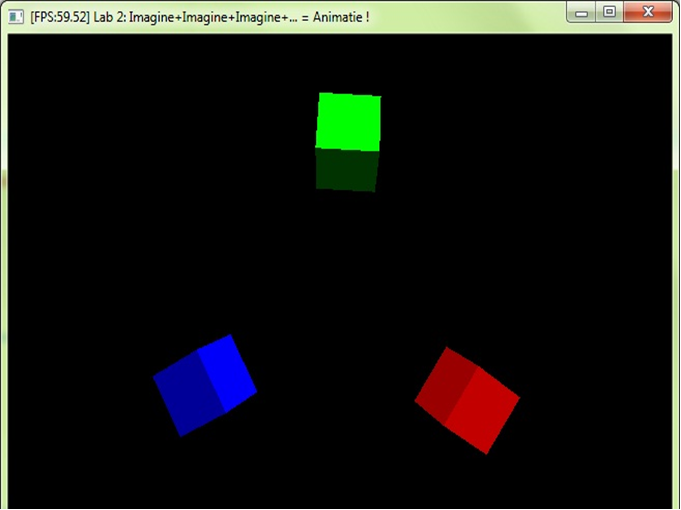
\includegraphics[width=0.48\textwidth]{l2f1a.png}
		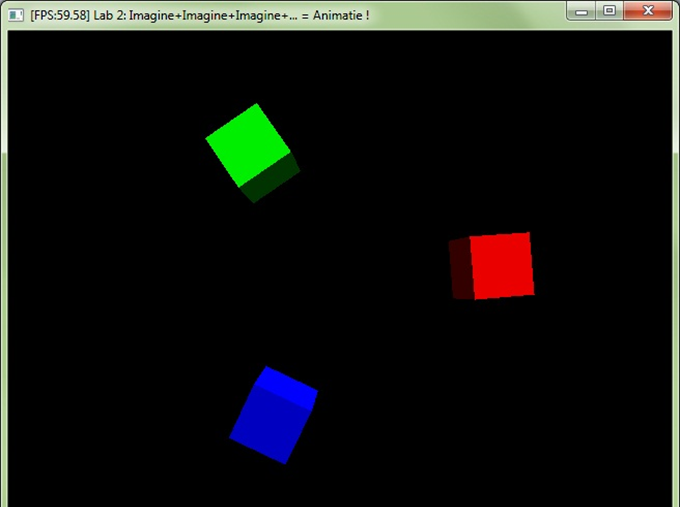
\includegraphics[width=0.48\textwidth]{l2f1b.png}
	\caption{Prima noastr\u a anima\c tie!}
	\label{fig:l2f1}
\end{figure}

\section{Elementele care determin\u a anima\c tia}
\^ In primul r\^ and ne vor trebui c\^ ateva variabile care s\u a con\c tin\u a deplasarea p\^ an\u a \^ in momentul curent.    
\begin{lstlisting}
    static float axisRot = 0.0f;
    static float globRotR = 0.0f;
    static float globRotG = 120.0f;
    static float globRotB = 240.0f;
\end{lstlisting}
Astfel avem o variabil\u a ce re\c tine rota\c tia \^ in jurul axei proprii, {\tt axisRot}, \^ impreun\u a cu alte $3$ variabile ce re\c tin rota\c tiile fiec\u arui cub \^ in jurul originii {\tt (globRotR, globRotG, globRotB)}. Arbitrar, am atribuit un caracter {\tt static} acestor va\-ria\-bi\-le; acest lucru face ca variabilele marcate cu {\tt static} s\u a \^ i\c si p\u astreze valorile de la o itera\c tie la alta. Acela\c si efect se putea ob\c tine \c si cu variabile globale. Urmeaz\u a afi\c sarea celor $3$ cuburi:
\begin{lstlisting}
    glColor3f(1.0f, 0.0f, 0.0f);
    glPushMatrix();
        glTranslatef(0.0f,0.0f,-20); //deplasat pe axele x, y, z
        glRotatef(globRotR, 0,0,1);
        glTranslatef(5.0f,0.0f,0.0f);
        glRotatef(axisRot,0,1,0); //rotit pe axa Y
        glutSolidCube(2); //cub cu latura 2
    glPopMatrix();
    
    glColor3f(0.0f, 1.0f, 0.0f);
    glPushMatrix();
        glTranslatef(0.0f,0.0f,-20); //deplasat pe axele x, y, z
        glRotatef(globRotG, 0,0,1);
        glTranslatef(5.0f,0.0f,0.0f);
        glRotatef(axisRot,0,1,0); //rotit pe axa Y
        glutSolidCube(2); //cub cu latura 2
    glPopMatrix();
    
    glColor3f(0.0f, 0.0f, 1.0f);
    glPushMatrix();
        glTranslatef(0.0f,0.0f,-20); //deplasat pe axele x, y, z
        glRotatef(globRotB, 0,0,1);
        glTranslatef(5.0f,0.0f,0.0f);
        glRotatef(axisRot,0,1,0); //rotit pe axa Y
        glutSolidCube(2); //cub cu latura 2
    glPopMatrix();
\end{lstlisting}
Este important de observat modul \^ in care sunt aplicate transform\u arile pe fiecare cub \^ in parte:
\begin{enumerate}
\item prima dat\u a cubul este deplasat cu $-20$ pe axa $Oz$ astfel \^ inc\^ at s\u a fie vizibil,
\item apoi se rote\c ste cubul cu un unghi,
\item datorit\u a rota\c tiei, transla\c tia aplicat\u a, $+5$ pe axa $Ox$, va fi conform\u a orient\u arii obiectului,
\item \^ inainte de a fi afi\c sat cubul se aplic\u a \c si o rota\c tie \^ in jurul axei sale.
\end{enumerate}
Dup\u a afi\c sarea celor $3$ cuburi, urmeaz\u a pasul de modificare a gradelor de rota\c tie folosite.
\begin{lstlisting}
    axisRot += 1.0f; axisRot=fmod(axisRot, 360.0f);
    globRotR += 0.5f; globRotR=fmod(globRotR, 360.0f);
    globRotG += 0.5f; globRotG=fmod(globRotG, 360.0f);
    globRotB += 0.5f; globRotB=fmod(globRotB, 360.0f);
\end{lstlisting}
Fiind variabile statice, acestea \^ i\c si p\u astreaz\u a valorile de la o itera\c tie la alta. Mai exact, aplic\^ and o incrementare, {\tt axisRot += 1.0f}, ob\c tinem o nou\u a rota\c tie care difer\u a de vechea rota\c tie cu un grad. 

Func\c tia {\tt fmod()} este echivalentul operatorului \%, dar ac\c tioneaz\u a asupra va\-ria\-bi\-le\-lor \^ in virgul\u a flotant\u a. Mai exact, {\tt fmod(a,b)} returneaz\u a restul, \^ in virgul\u a flotant\u a, a \^ imp\u ar\c tirii lui {\tt a} la {\tt b}. \^ In acest exemplu ne ajut\u a s\u a p\u astr\u am variabilele \^ in intervalul $[0, 360)$ grade.